\section{Particles of the Standard Model}%
\label{sec:sm_overview}

The particles of the SM are illustrated in~\Cref{fig:sm_particles}. They can be
broadly categorised into \emph{fermions} and \emph{bosons}, which are particles
with half-integer and integer spin, respectively. With the discovery of the
Higgs boson in 2012~\cite{HIGG-2012-27,CMS-HIG-12-028}, experimental evidence
for the existence of all SM particles is established.

% The SM, illustrated in, consists of 12 elementary
% spin-$\frac{1}{2}$ particles referred to as \emph{fermions} and their
% antiparticles, and five types of particles with integer spin referred to as
% \emph{bosons}. With the discovery of the Higgs boson in
% 2012~\cite{HIGG-2012-27,CMS-HIG-12-028}, experimental evidence for the existence
% of all particles predicted by the SM is established.

\begin{figure}[htbp]
  \centering

  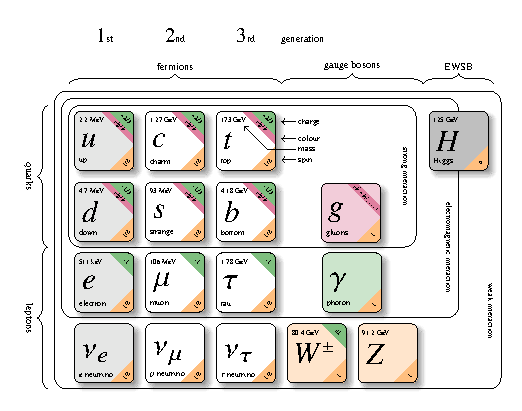
\includegraphics[width=\textwidth]{theory/sm}

  \caption{Particles of the SM. The diagram is adapted from Ref.~\cite{sm_tikz}
    with particle masses from Ref.~\cite{pdg2020}. Antifermions are not shown
    explicitly.  Not shown are the charges of the electroweak interaction, the
    weak isospin and weak hypercharge, which depend on the chirality of
    fermions. $*$: The gluons come in eight different states of colour charge
    which are combinations of colour and anticolour.}%
  \label{fig:sm_particles}
\end{figure}

An overview of the main categories of SM particles is given in the following:
\begin{description}

\item[Fermions] are massive\footnote{Neutrinos are considered as massless in the
    SM, however, the observation of neutrino
    oscillations~\cite{Super-Kamiokande:1998kpq,SNO:2002tuh} is experimental
    evidence for neutrinos having small but non-zero mass.} particles adhering
  to the Pauli exclusion principle, thus often referred to as \emph{matter}
  particles. For every fermion there exists a corresponding antifermion that has
  the same properties but with additive quantum numbers of opposite sign. The
  fermions of the SM are divided into \emph{quarks} that participate in the
  strong interaction, and \emph{leptons} that do not. They are further divided
  into up-type quarks ($u$, $c$, $t$), down-type quarks ($d$, $s$, $b$),
  electrically charged leptons ($e$, $\mu$, $\tau$), and neutrinos ($\nu_e$,
  $\nu_\mu$, $\nu_\tau$). The fermions come in three generations, the main
  difference between them being the mass of the fermions which increases with
  every successive generation. Consequently, all ordinary (stable) matter
  consists of fermions of the first generation: up-quarks, down-quarks, and
  electrons.

  The fermions carry charge-like quantum numbers that dictate the fundamental
  interactions they participate in. Quarks carry \emph{colour charge}, which
  comes in three discrete values of either \emph{red}, \emph{green}, or
  \emph{blue}, and the corresponding anticolours for antiquarks. Particles
  carrying colour charge take part in the strong interaction. Quarks and
  (electrically) charged leptons carry \emph{electric charge} and are therefore
  subject to the electromagnetic interaction. Fermions (antifermions) with
  left-handed (right-handed) chirality carry \emph{weak isospin}, therefore
  taking part in charged-current weak interactions. All fermions of the SM
  couple to the neutral-current weak interaction, the strength being determined
  by the weak isospin and the \emph{weak hypercharge} (or analogously the weak
  isospin and the electric charge, cf.~\Cref{seq:theory_ewk}).

\item[Gauge bosons] are particles with spin-$1$ and are therefore also referred
  to as vector bosons. Gauge bosons are the quanta of fields arising in quantum
  field theories built on certain symmetry principles, referred to as gauge
  theories, which will discussed in \Cref{sec:theo_symmetries_interactions}. The
  gauge bosons mediate strong, electromagnetic, and weak interaction through
  particle exchange.

  The (massless) gluons mediate the strong interaction through gluon exchange
  between particles with colour charge. Gluons are carriers of colour charge
  themselves, allowing self-interactions between gluons. The (massless) photon
  mediates the electromagnetic interaction between electrically charged
  particles. The gauge bosons of the weak interaction, the $W^\pm$ and
  $Z$~bosons, are the only massive gauge bosons in the SM. The $W^\pm$~bosons
  are electrically charged and mediate the charged-current weak interaction
  between particles carrying weak isospin. The neutral $Z$~boson mediates the
  neutral-current weak interaction.

\item[The Higgs boson] is the only scalar (spin-$0$) particle in the SM. The
  Higgs boson arises as part of the Brout--Englert--Higgs (BEH)
  mechanism~\cite{Englert:1964et,Higgs:1964pj} that is employed in the SM to
  generate the masses of fermions and massive gauge bosons ($W^\pm$ and $Z$)
  without violating the symmetry principles underlying the mathematical
  formulation of the SM. The Higgs boson and its role in the SM is discussed in
  \Cref{seq:theory_ewk}.

\end{description}

%%% Local Variables:
%%% mode: latex
%%% TeX-master: "../../phd_thesis"
%%% End:
